% !TEX TS-program = XeLaTeX
% !TeX root=main.tex
% دستورات زیر باید در اولین فایل پیوست باشند. آنها را حذف نکنید! در غیراینصورت در فهرست مطالب به جای عبارت پیوست عبارت فصل جلوی عنوان پیوست‌ها نمایش داده خواهد شد.
\addtocontents{toc}{
    \protect\renewcommand\protect\cftchappresnum{\appendixname~}%
    \protect\setlength{\cftchapnumwidth}{\mylenapp}}%
       
\chapter{آنچه باید بدانید}\label{App:App1}

در این بخش با نحوه مناسب درج منابع، نمونه مثالهایی از جدول، نمودار و الگوریتم در لاتک و همچنین امکانات دیگری از قالب \پ دانشگاه حکیم سبزواری آشنا خواهیم شد.



\section{ مدیریت مراجع با  \texorpdfstring{\lr{Bib\TeX}}{Bib\TeX} }
در بخش \ref{Sec:Ref} اشاره شد که با دستور 
 \lr{\textbackslash bibitem}
  می‌توان یک مرجع را تعریف نمود و با فرمان
 \lr{\textbackslash cite}
  به آن ارجاع داد. این روش برای تعداد مراجع زیاد و تغییرات آنها مناسب نیست. در ادامه به صورت مختصر توضیحی در خصوص برنامه \lr{BibTeX} که همراه با توزیع‌های معروف تِک عرضه می‌شود و نحوه استفاده از آن در زی‌پرشین خواهیم داشت.
  
یکی از روش‌های قدرتمند و انعطاف‌پذیر برای نوشتن مراجع مقالات و مدیریت مراجع در لاتک، استفاده از  \lr{BibTeX} 
 است.
 روش کار با  \lr{BibTeX} به‌این صورت است که مجموعه‌ی همه‌ی مراجعی را که در \پ استفاده کرده یا خواهیم کرد، 
در پرونده‌ی جداگانه‌ای نوشته و به آن فایل در سند خودمان به صورت مناسب لینک می‌دهیم.
 کنفرانس‌ها یا مجله‌های گوناگون برای نوشتن مراجع، قالب‌ها یا قراردادهای متفاوتی دارند که به آنها استیلهای مراجع گفته می‌شود.
 در این حالت به کمک ‌استیل‌های \lr{BibTeX} خواهید توانست تنها با تغییر یک پارامتر در پرونده‌ی ورودی خود، مراجع را مطابق قالب موردنظر تنظیم کنید. 
 بیشتر مجلات و کنفرانس‌های معتبر یک پرونده‌ی سبک (\lr{BibTeX Style}) با پسوند \lr{bst} در وب‌گاه خود می‌گذارند که برای همین منظور طراحی شده است.

به جز نوشتن مقالات این سبک‌ها کمک بسیار خوبی برای تهیه‌ی مستندات علمی همچون پایان‌نامه‌هاست که فرد می‌تواند هر قسمت از کارش را که نوشت مراجع مربوطه را به بانک مراجع خود اضافه نماید. با داشتن چنین بانکی از مراجع، وی خواهد توانست به راحتی یک یا چند ارجاع به مراجع و یا یک یا چند بخش را حذف یا اضافه ‌نماید؛ 
مراجع به صورت خودکار مرتب شده و فقط مراجع ارجاع داده شده در قسمت کتاب‌نامه خواهندآمد. قالب مراجع به صورت یکدست مطابق سبک داده شده بوده و نیازی نیست که کاربر درگیر قالب‌دهی به مراجع باشد. 

در حال حاضر چندین قالب (استیل یا سبک) فارسی قابل استفاده هستند که از بین آنها قالب
\lr{unsrt-fa} 
مطابق با یکی از روش‌هایی است که در دستورالعمل نگارش پایان‌نامه دانشگاه حکیم سبزواری برای درج مراجع آمده است: روش درج منابع به ترتیب ارجاع در متن. در فایل 
\lr{main}
از این استیل استفاده شده است.

با استفاده از استیل فوق می‌توانید به انواع مختلفی از مراجع فارسی و لاتین ارجاع دهید. به عنوان نمونه مرجع 
\cite{Omidali82phdThesis}
 یک نمونه پروژه دکترا (به فارسی) و مرجع 
\cite{Vahedi87} یک نمونه مقاله مجله فارسی است.
مرجع 
\cite{Amintoosi87afzayesh}  یک نمونه  مقاله کنفرانس فارسی و
مرجع 
\cite{Pedram80osool} یک نمونه کتاب فارسی با ذکر مترجمان و ویراستاران فارسی است. مرجع 
\cite{Khalighi07MscThesis} یک نمونه پروژه کارشناسی ارشد انگلیسی و
\cite{Khalighi2015xepersian} هم یک نمونه متفرقه  می‌باشند.

مراجع 
\cite{Gonzalez02book,Baker02limits} 
نمونه کتاب و مقاله انگلیسی هستند.


\subsection{ نحوه استفاده از سبک‌های فارسی}


برای استفاده از بیب‌تک باید مراجع خود را در یک فایل با پسوند \lr{bib} ذخیره نمایید. یک فایل \lr{bib} در واقع یک پایگاه داده از مراجع\LTRfootnote{Bibliography Database}  شماست که هر مرجع در آن به عنوان یک رکورد از این پایگاه داده
با قالبی خاص ذخیره می‌شود. به هر رکورد یک مدخل\LTRfootnote{Entry} گفته می‌شود. یک نمونه مدخل برای معرفی کتاب \lr{Digital Image Processing} در ادامه آمده است:

\singlespacing
\begin{LTR}
\begin{verbatim}
@BOOK{Gonzalez02image,
  AUTHOR =      {Rafael Gonzalez and Richard Woods},
  TITLE =       {Digital Image Processing},
  PUBLISHER =   {Prentice-Hall, Inc.},
  YEAR =        {2006},
  EDITION =     {3rd},
  ADDRESS =     {Upper Saddle River, NJ, USA}
}
\end{verbatim}
\end{LTR}
\doublespacing

در مثال فوق، \lr{@BOOK} مشخصه‌ی شروع یک مدخل مربوط به یک کتاب و \lr{Gonzalez02book} برچسبی است که به‌این مرجع منتسب شده است.
 این برچسب بایستی یکتا باشد. برای آنکه فرد به راحتی بتواند برچسب مراجع خود را به خاطر بسپارد و حتی‌الامکان برچسب‌ها متفاوت با هم باشند معمولاً از قوانین خاصی به‌این منظور استفاده می‌شود. یک قانون می‌تواند فامیل نویسنده‌ی اول+دورقم سال نشر+اولین کلمه‌ی عنوان اثر باشد. به \lr{AUTHOR} و $\dots$ و \lr{ADDRESS} فیلدهای این مدخل گفته می‌شود؛ که هر یک با مقادیر مربوط به مرجع مقدار گرفته‌اند. ترتیب فیلدها مهم نیست. 

انواع متنوعی از مدخل‌ها برای اقسام مختلف مراجع همچون کتاب، مقاله‌ی کنفرانس و مقاله‌ی ژورنال وجود دارد که برخی فیلدهای آنها با هم متفاوت است. 
نام فیلدها بیانگر نوع اطلاعات آن می‌باشد. مثالهای ذکر شده در فایل \lr{MyReferences.bib} کمک خوبی به شما خواهد بود. 
%این فایل یک فایل متنی بوده و با ویرایشگرهای معمول همچون \lr{Notepad++} قابل ویرایش می‌باشد. برنامه‌هایی همچون 
%\lr{TeXMaker}
% امکاناتی برای نوشتن این مدخل‌ها دارند و به صورت خودکار فیلدهای مربوطه را در فایل \lr{bib}  شما قرار می‌دهند.  
با استفاده از سبک‌های فارسی آماده شده، محتویات هر فیلد می‌تواند به فارسی نوشته شود، ترتیب مراجع و نحوه‌ی چینش فیلدهای هر مرجع را سبک مورد استفاده  مشخص خواهد کرد.

%نکته: بدون اعمال تنظیمات موردنیاز \lr{Bib\TeX} در \lr{TeXWorks}، مراجع فارسی در استیل‌هایی که مراجع را به صورت مرتب شده چاپ می‌کنند، ترتیب کاملاً درستی نخواهند داشت. برای توضیحات بیشتر \cite{persianbib87userguide} را ببینید یا به سایت پارسی‌لاتک مراجعه فرمایید. تنظیمات موردنیاز در \lr{TeXMaker} اصلاح شده اعمال شده‌اند. برای درج مراجع خود لازم نیست نگران موارد فوق باشید. 

برای عمل به‌این روش: 
\textbf{در فایل 
\lr{MyReferences.bib}
 که همراه با این \پ هست، موارد مختلفی درج شده است، کافیست مراجع خود را جایگزین موارد مندرج در آن نمایید.
}

پس از قرار دادن مراجع خود، یک بار \lr{XeLaTeX} را روی سند خود اجرا نمایید، سپس \lr{bibtex} و پس از آن دوبار \lr{XeLaTeX} را. 
در 
\lr{TeXstudio} و
\lr{TeXMaker} کلید \lr{F11} و در \lr{TeXWorks} هم گزینه‌ی \lr{BibTeX} از منوی \lr{Typeset}، \lr{BibTeX} را روی سند شما اجرا می‌کنند.

برای بسیاری از مقالات لاتین حتی لازم نیست که مدخل مربوط به آنرا خودتان بنویسید. با جستجوی نام مقاله + کلمه \lr{bibtex}  در اینترنت سایتهای بسیاری همچون \lr{ACM} و \lr{ScienceDirect} را خواهید یافت که مدخل \lr{bibtex} مربوط به مقاله شما را دارند و کافیست آنرا به انتهای فایل \lr{MyReferences} اضافه کنید.

%از هر یک از سبکهای \lr{Persian-bib} می‌توانید استفاده کنید، البته اگر از سه استیل آخر استفاده می‌کنید و مایلید که مراجع شما شماره بخورند باید بسته \lr{natbib} را با گزینه \lr{numbers} فراخوانی نمایید.

\section{جدول}
رسم جدول نیز در لاتک کار سختی نیست.  جدول 
\eqref{tab:MotionModels}
مدل‌های تبدیل را نشان می‌دهد.

\begin{table}[ht]
\caption{مدلهای تبدیل.}
\label{tab:MotionModels}
\centering
\onehalfspacing
\begin{tabular}{|r|c|l|r|}
\hline نام مدل & درجه آزادی & تبدیل مختصات & توضیح \\ 
\hline انتقالی & ۲ & $\begin{aligned} x'=x+t_x \\ y'=y+t_y \end{aligned}$  &  انتقال دوبعدی\\ 
\hline اقلیدسی & ۳ & $\begin{aligned} x'=xcos\theta - ysin\theta+t_x \\ y'=xsin\theta+ycos\theta+t_y \end{aligned}$  &  انتقالی+دوران \\ 
\hline 
\end{tabular} 
\end{table}




\section{درج الگوریتم}
\subsection{الگوریتم با دستورات فارسی}
 الگوریتم 
 \eqref{alg:DLT} 
 یک الگوریتم با دستورات فارسی است.
\begin{algorithm}[t]
\onehalfspacing
\caption{الگوریتم \lr{DLT} برای تخمین ماتریس هوموگرافی.} \label{alg:DLT}
\begin{algorithmic}[1]
\REQUIRE $n\geq4$ زوج نقطهٔ متناظر در دو تصویر 
${\mathbf{x}_i\leftrightarrow\mathbf{x}'_i}$
\\
\ENSURE ماتریس هوموگرافی $H$ به نحوی‌که: 
$\mathbf{x}'_i = H \mathbf{x}_i$.
  \STATE برای هر زوج نقطهٔ متناظر
$\mathbf{x}_i\leftrightarrow\mathbf{x}'_i$ 
ماتریس $\mathbf{A}_i$ را با استفاده از رابطهٔ \ref{eq:DLT_Ah} محاسبه کنید.
  \STATE ماتریس‌های ۹ ستونی  $\mathbf{A}_i$ را در قالب یک ماتریس $\mathbf{A}$ ۹ ستونی ترکیب کنید. 
  \STATE تجزیهٔ مقادیر منفرد \lr{(SVD)}  ماتریس $\mathbf{A}$ را بدست آورید. بردار واحد متناظر با کمترین مقدار منفرد جواب $\mathbf{h}$ خواهد بود.
  \STATE  ماتریس هوموگرافی $H$ با تغییر شکل $\mathbf{h}$ حاصل خواهد شد.
\end{algorithmic}
\end{algorithm}

\subsection{الگوریتم با دستورات لاتین}
الگوریتم
 \ref{alg:RANSAC}
  یک الگوریتم با دستورات لاتین است.

\begin{algorithm}[t]
\onehalfspacing
\caption{الگوریتم \lr{RANSAC} برای تخمین ماتریس هوموگرافی.} \label{alg:RANSAC}
\begin{latin}
\begin{algorithmic}[1]
\REQUIRE $n\geq4$ putative correspondences, number of estimations, $N$, distance threshold $T_{dist}$.\\
\ENSURE Set of inliers and Homography matrix $H$.
\FOR{$k = 1$ to $N$}
  \STATE Randomly choose 4 correspondence,
  \STATE Check whether these points are colinear, if so, redo the above step
  \STATE Compute the homography $H_{curr}$ by DLT algorithm from the 4 points pairs,
  \STATE $\ldots$ % الگوریتم کامل نیست
  \ENDFOR
  \STATE Refinement: re-estimate H from all the inliers using the DLT algorithm.
\end{algorithmic}
\end{latin}
\end{algorithm}

%
%\section{تصویر}
%نمونه تصاویری در بخش قبل دیدیم. دو تصویر شیر کنار هم را هم در شکل \ref{fig:twolion} مشاهده می‌کنید.
%\begin{figure}[t]
%\centering 
%\subfigure[شیر ۱]{ \label{fig:twolion:one}
%\includegraphics[width=.3\textwidth]{lion}}
%%\hspace{2mm}
%\subfigure[شیر ۲]{ \label{fig:twolion:two}
%\includegraphics[width=.3\textwidth]{lion}}
%\caption{دو شیر}
%\label{fig:twolion} %% label for entire figure
%\end{figure}



\section{درج کد}
درج کد به زبانهای مختلف نیز به سادگی امکان‌پذیر است. برنامه 
\ref{Code:MATLAB1}
یک قطعه کد \lr{MATLAB} را نشان می‌دهد.
\singlespacing
%\begin{figure}
%\begin{latin}
\begin{lstlisting}[language=MATLAB,breaklines=true,numbers=right, numberstyle=\footnotesize, numbersep=-10pt,  frame=single, breakatwhitespace=false,
caption={نمونه کد \lr{MATLAB}},label={Code:MATLAB1}]
% define a continuous function
f = '4*sin(2*pi*t)';
ezplot(f);
for i=1:10
    disp(i)
end
\end{lstlisting}
%\end{latin}


%\end{figure}
\doublespacing


\section{فرمول‌های ریاضی}
تقریباً هر آنچه دانشجویان برای نوشتن فرمول‌های ریاضی لازم دارند، در کتاب 
\lr{mathmode}
آمده است. کافیست در خط فرمان دستور زیر را وارد کنید:
\begin{latin}
texdoc mathmode
\end{latin}
متن زیر یک متن شامل انواعی از اشیاء ریاضی است که با ملاحظه فایل \lr{.tex} این سند می‌توانید دستورات مربوطه را مشاهده فرمایید.

شناخته‌شده‌ترین روش تخمین ماتریس هوموگرافی الگوریتم تبدیل خطی مستقیم 
%(\lr{DLT\LTRfootnote{Direct Linear Transform}}) 
است.  فرض کنید چهار زوج نقطهٔ متناظر در دو تصویر در دست هستند،  $\mathbf{x}_i\leftrightarrow\mathbf{x}'_i$   و تبدیل با رابطهٔ
  $\mathbf{x}'_i = H\mathbf{x}_i$
  نشان داده می‌شود که در آن:
\[\mathbf{x}'_i=(x'_i,y'_i,w'_i)^\top  \]
و $H$ ماتریس تبدیل است.
رابطه زیر را برای الگوریتم  \eqref{alg:DLT} لازم دارم.
\begin{equation}\label{eq:DLT_Ah}
\left[
\begin{array}{ccc}
0^\top & -w'_i\mathbf{x}_i^\top & y'_i\mathbf{x}_i^\top \\ 
w'_i\mathbf{x}_i & 0^\top & -x'_i\mathbf{x}_i^\top \\ 
- y'_i\mathbf{x}_i^\top & x'_i\mathbf{x}_i^\top & 0^\top
\end{array} 
\right]
\left(
\begin{array}{c}
\mathbf{h}^1 \\ 
\mathbf{h}^2 \\ 
\mathbf{h}^3
\end{array} 
\right)=0
\end{equation}

\section{نمودار}

%\setRTLparagraphfootnotes
لاتک بسته‌هایی با قابلیت‌های زیاد برای رسم انواع مختلف نمودارها دارد. مانند بسته‌های \lr{Tikz} و  \lr{PSTricks}. توضیح اینها فراتر از این پیوست کوچک است.
% مثالهایی از رسم نمودار را در مجموعه پارسی‌لاتک خواهید یافت. 
\footnote{
نمونه مثالهایی از بسته \lr{Tikz} را می‌توانید
 در \url{http://www.texample.net/tikz/examples/} ببینید. به دانشجویانی که قصد قرار دادن اشکالی همانند گراف در سند خود را دارند، توصیه می‌شود مثالهایی از سایت مذکور را ملاحظه فرمایند.}
یک نمونه نمودار رسم شده با بسته‌ی 
\lr{TikZ}
 در شکل 
\ref{fig:parabola}
نشان داده شده است.
\begin{figure}[t]
\centering
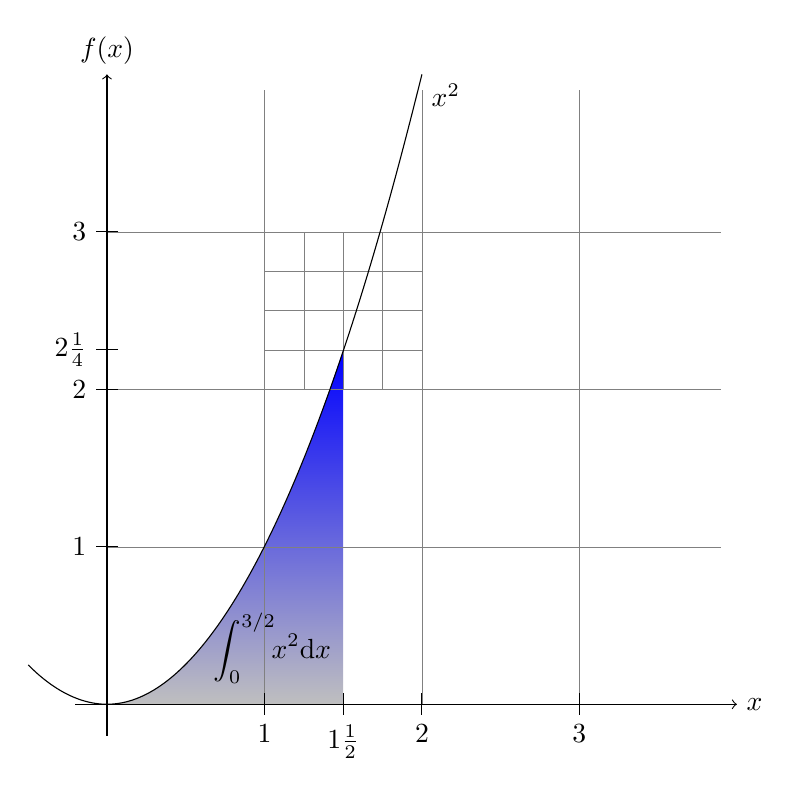
\begin{tikzpicture}[scale=2]
  \shade[top color=blue,bottom color=gray!50] 
      (0,0) parabola (1.5,2.25) |- (0,0);
  \draw (1.05cm,2pt) node[above] 
      {$\displaystyle\int_0^{3/2} \!\!x^2\mathrm{d}x$};

  \draw[style=help lines] (0,0) grid (3.9,3.9)
       [step=0.25cm]      (1,2) grid +(1,1);

  \draw[->] (-0.2,0) -- (4,0) node[right] {$x$};
  \draw[->] (0,-0.2) -- (0,4) node[above] {$f(x)$};

  \foreach \x/\xtext in {1/1, 1.5/1\frac{1}{2}, 2/2, 3/3}
    \draw[shift={(\x,0)}] (0pt,2pt) -- (0pt,-2pt) node[below] {$\xtext$};

  \foreach \y/\ytext in {1/1, 2/2, 2.25/2\frac{1}{4}, 3/3}
    \draw[shift={(0,\y)}] (2pt,0pt) -- (-2pt,0pt) node[left] {$\ytext$};

  \draw (-.5,.25) parabola bend (0,0) (2,4) node[below right] {$x^2$};
\end{tikzpicture}
\caption{یک نمودار زیبا با ارقام فارسی و قابلیت بزرگ‌نمایی بسیار، بدون از دست دادن کیفیت.}
\label{fig:parabola}
\end{figure}
موقعبت قرارگیری اشیاء شناور مانند جدول و تصویر توسط خود لاتک مدیریت می‌شود. گاهی موقعیت مناسب پیدا نمی‌شود و این موارد در بافر قرار می‌گیرند و در انتهای بخش یا فصل نمایش داده می‌شوند. برای ملزم کردن لاتک به نمایش اشیايی که در بافر دارد کافیست از دستور 
\verb!\clearpage!
استفاده کنیم.

 گاهی  ممکن است لازم باشد خودمان دستور رفتن به صفحه جدید را با دستور 
\verb!\newpage!
به لاتک بدهیم، مثل الان ...
\newpage




\section{درج توضیحات در حاشیه}
%\setLTRparagraphfootnotes
فراگیر شدن اینترنت ارتباطات از راه دور را سهل نموده است. فرض کنید دانشجو \پ خود را نوشته و از طریق اینترنت برای اظهار نظر به استاد راهنمای خود رسانده است. اگر قرار باشد استاد راهنما پس از مطالعه \پ، مواردی را  گوشزد نماید، به جز راه‌های معمول (تلفن و ایمیل و ...) یک راهکار مناسب استفاده از بسته 
\lr{todonotes}
در لاتک است. به کمک این بسته که جناب آقای خلیقی از نسخه ۱۶ بسته
\lr{bidi}
امکان استفاده از آن‌را برای فارسی‌زبانان فراهم نموده‌اند، به راحتی می‌توان با استفاده از دستور
\verb!\todo{NOTE}!
نکته، یا نکات موردنظر  را در حاشیه متن یادداشت کرد.  
\todo{
توضیح بیشتری لازم است.
}

مثلاً استاد راهنما از دانشجو بخواهد که در بخشی توضیح بیشتری داده شود. استاد راهنما یا داور می‌تواند حتی محل پیشنهادی برای درج یک تصویر را به راحتی برای دانشجو مشخص کند.
\missingfigure[figwidth=\textwidth,figcolor=white]{یک تصویر از خروجی الگوریتم 
 \ref{alg:RANSAC}
را در اینجا قرار دهید.}

نکته قابل توجه آن است که‌این توضیحات حاشیه‌ای فقط در نسخه پیش‌نویس قابل دیدن هستند و در نسخه نهایی، نمایش داده نخواهند شد (به بخش 
\ref{Sec:draft}
مراجعه شود).
\todo[fancyline,color=green!30]{مرجع این مطلب؟}
بسته 
\lr{todonotes}
امکانات بسیاری دارد که با ملاحظه راهنمای آن می‌توانید با آنها آشنا شوید. برای دیدن راهنما کافیست در خط فرمان دستور زیر را اجرا کنید:

\begin{latin}	
texdoc todonotes
\end{latin}	
یکی دیگر از امکانات این بسته آن است که می‌توان فهرست نکات را در ابتدای سند داشت.  قالب \پ دانشگاه حکیم سبزواری به نحوی آماده شده است که فقط در حالت پیش‌نویس این فهرست پس از فهرست مطالب نمایش داده می‌شود.



\section{حالت پیش‌نویس}\label{Sec:draft}
یکی از امکانات جالب قالب پایان‌نامه دانشگاه حکیم سبزواری امکان استفاده از حالت پیش‌نویس 
\lr{(draft)}
است. هنگامی‌که سند شما در حالت پیش‌نویس باشد:

\singlespacing
\begin{enumerate}
\item 
هیچ یک از صفحات آغازین پایان‌نامه، تا فهرست مطالب نمایش داده نمی‌شود (به جز صفحه اول).
\item
روی صفحه اول عبارت «پیش‌نویس» به صورت درشت و کم‌رنگ نمایش داده می‌شود.
\item
تمام پیوندها شامل لینک به فصلها، بخشها، مراجع و فرمولها به صورت رنگی نمایش داده می‌شود.
\item
فهرست نکات درج شده توسط
\lr{todo}
پس از فهرست اصلی و با عنوان «فهرست کارهای باقیمانده» نمایش داده می‌شود.
\item
شماره صفحاتی که به هر مرجع ارجاع داده شده است در بخش مراجع نمایش داده می‌شود.
\end{enumerate}
\doublespacing
هر یک از موارد بالا تا زمانی که نسخه نهایی \پ نیاز نباشد بسیار مورد توجه و مفید می‌باشند. 
 اگر حالت پیش‌نویس فعال نباشد، متن به صورتی که مناسب چاپ باشد نمایش داده می‌شود.

برای استفاده از حالت پیش‌نویس باید گزینه 
\lr{draft}
به دستور 
\lr{documentclass}
در ابتدای فایل 
\lr{main}
اضافه شود. اگر وضعیت فعلی این دستور به صورت زیر است:
\begin{latin} \noindent
\verb!\documentclass[oneside,openany,dvipsnames,msc,12pt]{HSU-Thesis}!
\end{latin}
باید به صورت زیر در بیاید:
\begin{latin} \noindent
\verb!\documentclass[oneside,openany,dvipsnames,msc,12pt,draft]{HSU-Thesis}!
\end{latin}

به صورت پیش‌فرض، حالت پیش‌نویس غیرفعال است که در صورت نیاز باید آنرا به صورت فوق فعال نموده و خروجی را مشاهده فرمایید.  شکل 
\ref{fig:draft}
تصویری از یک متن را در حالت معمولی و در حالت پیش‌نویس نشان می‌دهد.
\begin{figure}[t]
\centering 
\subfigure[حالت پیش‌فرض]{ \label{fig:draft:no}
\includegraphics[width=.445\textwidth]{nodraft}}
\subfigure[حالت پیش‌نویس]{ \label{fig:draft:yes}
\includegraphics[width=.53\textwidth]{draft}}
\caption[مقایسه حالت معمولی و حالت پیش‌نویس]
{مقایسه خروجی بخشی از نوشتار در حالت پیش‌فرض (بدون استفاده از گزینه 
\lr{draft}) و حالت پیش‌نویس
\lr{(draft)}}
\label{fig:draft} %% label for entire figure
\end{figure}

%\newpage
%\setLTRparagraphfootnotes
%در اینجا یک زیرنویس چپ به راست را امتحان می‌کنم
%\LTRfootnote{Footnote}.

